% !TEX program = pdflatex
% MDPI Education Sciences
\documentclass[applsci,article,submit,pdftex,moreauthors]{Definitions/mdpi}
\usepackage{tabularx}

% ---------- MDPI metadata ----------
\firstpage{1}
\makeatletter
\setcounter{page}{\@firstpage}
\makeatother
\pubvolume{16}
\issuenum{11}
\articlenumber{XXXX}
\pubyear{2026}
\copyrightyear{2026}
\datereceived{XX Month 2026}
\dateaccepted{XX Month 2026}
\datepublished{XX Month 2026}

% ---------- Title ----------
\Title{Temporal Attention-Enhanced Lightweight CNN for Student Engagement Detection on Edge Devices}

% ---------- Authors ----------
\Author{Donghai Peng $^{1}$ and Huanjie Yu $^{2,}$*}
\AuthorNames{Donghai Peng and Huanjie Yu}
\address{%
$^{1}$ \quad School of Information Engineering, Shaoguan University, Shaoguan, Guangdong 512005, China\\
$^{2}$ \quad School of Computer Science, Hunan University of Technology and Business, Changsha, Hunan 410205, China}
\corres{Correspondence: semhaqx@gmail.com}

% ---------- Abstract (English) ----------
\abstract{%
Automated student engagement detection from facial expressions is a promising approach for real-time monitoring in educational environments.
This paper proposes a lightweight deep learning framework integrating MobileNetV3 and EfficientNet-B0 with a multi-scale Channel-Spatial Attention Module (CSAM), focal weighted loss, and a BiLSTM-based temporal aggregation module for engagement recognition.
Our multi-scale CSAM employs parallel 3$\times$3, 5$\times$5, and 7$\times$7 convolutions with adaptive fusion weights to capture facial features at multiple spatial scales, enabling more robust detection of subtle engagement cues.
For video-level prediction, we introduce a temporal aggregation module comprising a bidirectional long short-term memory (BiLSTM) network~\cite{hochreiter1997lstm,schuster1997bilstm} for frame sequence encoding and attention-weighted temporal pooling, which learns to emphasize engagement-relevant temporal segments.
We map the FER2013 facial expression dataset (35,887 images) and CK+ dataset (804 images) to a four-class engagement taxonomy (Engaged, Boredom, Frustration, Confusion) via an emotion-to-engagement mapping grounded in affective computing literature.
Our training pipeline combines two-stage transfer learning from ImageNet, data augmentation, focal weighted loss with label smoothing, and weighted sampling for joint class balancing and hard-example mining.
MobileNetV3+CSAM achieves 70.5\% accuracy on the four-class frame-level task with 1.26M parameters and 0.068G FLOPs---a 19.6$\times$ energy reduction compared to VGG-16.
EfficientNet-B0+CSAM reaches 69.1\% with 5.4M parameters.
CSAM outperforms existing attention mechanisms (SE-Net, ECA-Net, CBAM) by 2.4--3.7\% on the same backbone.
Ablation studies confirm the contributions of data augmentation (+3.8\%), focal weighted loss (+1.5--2.4\% F1 on minority classes), transfer learning (+9.2\%), and focal loss parameter selection ($\gamma=1.0$ outperforms $\gamma=2.0$ by 0.9\% F1).
Cross-dataset evaluation on CK+ (71.9\% accuracy without fine-tuning, 114 test samples) provides preliminary evidence of generalizability.
On DAiSEE, frame-level binary engagement classification achieves 61.2\% accuracy (44.0\% macro F1), while our temporal aggregation pipeline combining MobileNetV3+CSAM frame features with BiLSTM-based temporal modeling achieves 94.8\% video-level accuracy and 48.7\% macro F1. Given DAiSEE's extreme class imbalance (\~94\% Engaged), a majority-class baseline achieves 94.0\% accuracy with 0\% Disengaged F1; our model achieves 35.6\% Disengaged F1, demonstrating that temporal modeling meaningfully improves disengagement detection beyond trivial baselines.
The complete pipeline maintains edge deployment feasibility, processing video clips in real time on resource-constrained devices.
These results establish that engagement detection is fundamentally a temporal problem, and that lightweight CNN frame encoders combined with efficient temporal aggregation offer a practical solution for real-world classroom monitoring.
}

\keyword{edge computing; student engagement; facial expression recognition; MobileNetV3; lightweight CNN; attention mechanism; temporal modeling; BiLSTM; video analysis; real-time inference}

% ---------- Chinese abstract ----------






\begin{document}

\section{Introduction}

Student engagement is one of the strongest predictors of academic success and learning outcomes. Engaged students show greater attention, participation, and persistence, all of which support deeper learning~\cite{fredricks2004school,dixson2015measuring}. Yet monitoring engagement in real time remains a persistent challenge for educators, particularly in large classes and online settings where manual observation is impractical~\cite{whitehill2014faces}. The expansion of online and blended education has further increased the need for automated, scalable engagement monitoring tools~\cite{savchenko2022emotions}.

Computer vision offers a promising avenue: facial expressions encode cognitive and emotional states, including interest, confusion, boredom, and frustration, that correlate with engagement levels~\cite{kleinsmith2013affective,jampour2022multiview}. Convolutional neural networks (CNNs) have advanced facial expression recognition substantially~\cite{bengio2013representation}, yet deploying them in real classroom environments faces practical computational constraints. Models such as ResNet-50 and VGG-16 demand memory and processing power that exceed the capacity of edge devices commonly available in schools~\cite{howard2017mobilenets}. This gap between recognition accuracy and deployability on resource-limited hardware motivates the search for efficient architectures suitable for classroom use.

While prior work has demonstrated the feasibility of CNN-based engagement detection~\cite{whitehill2014faces,tonguc2020automatic,savchenko2022emotions}, four gaps remain\label{sec:intro_gaps}. First, most existing methods employ heavyweight architectures (ResNet-50, VGG-16) that are impractical for real-time classroom deployment on edge devices. Second, attention mechanisms designed for large backbones (e.g., CBAM~\cite{woo2018cbam}) have not been specifically adapted for mobile-class architectures used in engagement detection, and existing spatial attention typically uses a single receptive field, missing multi-scale facial cues. Third, class imbalance in engagement datasets---where disengaged states are underrepresented---is typically addressed with simple class weighting rather than joint hard-example mining and balanced sampling. Fourth, most frame-level approaches treat each image independently, ignoring the temporal dynamics inherent in video-based engagement detection. Engagement states fluctuate over time, and aggregating predictions across video segments can substantially improve detection accuracy~\cite{yue2015beyond}.

To address these gaps, this paper investigates lightweight deep learning architectures for student engagement detection. Specifically, we evaluate MobileNetV3~\cite{howard2019mobilenetv3} and EfficientNet-B0~\cite{tan2019efficientnet}, which are designed to achieve competitive accuracy while maintaining low computational overhead. We repurpose the FER2013 facial expression dataset~\cite{goodfellow2013challenges} and CK+~\cite{lucey2010ck} for engagement detection through an emotion-to-engagement mapping, converting the seven basic emotions into four engagement states (Engaged, Boredom, Frustration, Confusion).

The main contributions of this paper are as follows:
\begin{enumerate}
\item We propose a lightweight CNN framework integrated with a multi-scale Channel-Spatial Attention Module (CSAM), which employs parallel 3$\times$3, 5$\times$5, and 7$\times$7 convolutions with adaptive fusion weights to capture facial features at multiple spatial scales. CSAM is designed specifically for mobile architectures with compact channel attention (reduction ratio $r=4$) and per-block feature recalibration. CSAM outperforms existing attention mechanisms (SE-Net, ECA-Net, CBAM) by 2.4--3.7\% on the same backbone, with only 0.3\% parameter overhead.
\item We introduce a temporal aggregation module comprising a bidirectional LSTM (BiLSTM)~\cite{hochreiter1997lstm,schuster1997bilstm} for frame sequence encoding and attention-weighted temporal pooling for video-level engagement prediction. On DAiSEE, this module achieves 94.8\% video-level accuracy and 48.7\% macro F1. Given DAiSEE's extreme class imbalance (\~94\% Engaged), the meaningful improvement is in Disengaged-class F1 (35.6\% vs.\ 21.9\% frame-level), and the BiLSTM + attention pooling outperforms simpler temporal strategies by 3.8--4.2\% Disengaged F1, demonstrating that learned temporal attention is critical for engagement detection.
\item We introduce a focal weighted loss function with label smoothing and gradient clipping that jointly addresses class imbalance and hard-example mining, outperforming standard weighted cross-entropy by 1.5\% F1 on Boredom and 2.4\% F1 on Confusion. We further employ weighted sampling to ensure balanced class representation during training.
\item We repurpose FER2013 and CK+ for engagement detection through an emotion-to-engagement mapping grounded in affective computing theory, enabling evaluation on publicly available datasets with well-established benchmarks.
\item We conduct comprehensive deployment-oriented experiments comparing lightweight models with heavier architectures, demonstrating that MobileNetV3+CSAM achieves 70.5\% accuracy with only 1.26M parameters and 0.068G FLOPs, offering an optimal accuracy-efficiency trade-off. The complete temporal pipeline maintains edge deployment feasibility.
\end{enumerate}

The remainder of this paper is organized as follows. Section~\ref{sec:related} reviews related work on engagement detection and lightweight CNN architectures. Section~\ref{sec:method} describes the proposed methodology and presents the experimental results. Section~\ref{sec:discussion} discusses the findings and limitations. Section~\ref{sec:conclusion} concludes the paper.

%%%%%%%%%%%%%%%%%%%%%%%%%%%%%%%%%%%%%%%%%%
\section{Related Work}
\label{sec:related}

\subsection{Student Engagement Detection}

Student engagement is a multidimensional construct encompassing behavioral, emotional, and cognitive components~\cite{fredricks2004school}. Behavioral engagement refers to participation and effort, emotional engagement encompasses affective reactions such as interest, boredom, and frustration, and cognitive engagement involves self-regulation and investment in learning~\cite{skinner2009motivational}. Early approaches to automatic engagement detection relied on behavioral cues such as gaze direction, head pose, and body posture~\cite{whitehill2014faces}. Whitehill et al.~\cite{whitehill2014faces} pioneered the use of facial expressions for engagement recognition, demonstrating that computer vision systems can achieve reasonable accuracy in distinguishing engaged from disengaged states.

CNN-based approaches now dominate engagement detection. Learning analytics research has similarly explored engagement detection from clickstream and interaction data~\cite{baker2014educational}, establishing engagement monitoring as a core application of educational data mining. Tongu\c{c} and Ozkara~\cite{tonguc2020automatic} recognized student emotions during lectures, surpassing traditional machine learning baselines. Santoni et al.~\cite{santoni2023cnn} tackled class imbalance in the DAiSEE dataset through CNN models with data augmentation. Grafsgaard et al.~\cite{grafsgaard2013automatically} demonstrated that facial expression features can predict engagement and frustration in tutoring interactions. Bosch et al.~\cite{bosch2015automatic} investigated automatic recognition of facial action units as indicators of engagement. Monkaresi et al.~\cite{monkaresi2017automated} combined facial expression detection with heart rate monitoring for automated engagement detection. D'Mello and Graesser~\cite{dmello2012auto} characterized confusion as a productive learning emotion, providing theoretical grounding for the Confusion engagement class. Dewan et al.~\cite{dewan2019deep} reviewed deep learning approaches for engagement detection in online learning environments.

Recent work has explored various deep learning architectures for engagement detection. Savchenko et al.~\cite{savchenko2022emotions} proposed a deep learning framework for student engagement classification in online learning environments. Nezami et al.~\cite{nezami2020automatic} developed a video-based platform integrating emotion detection to increase online learning engagement. Kaur and Kaur~\cite{kaur2022review} applied CNN-based facial expression recognition for engagement evaluation in classroom settings. Yu et al.~\cite{yu2024bridging} investigated engagement and attention level detection on the DAiSEE dataset using various deep learning approaches.

\subsection{Theoretical Foundations of Student Engagement}
\label{sec:theory}

Our emotion-to-engagement mapping is grounded in three complementary theoretical frameworks from educational psychology. First, Csikszentmihalyi's flow theory~\cite{csikszentmihalyi1990flow} describes optimal engagement as a state of deep immersion characterized by focused concentration and intrinsic motivation. In the flow state, learners exhibit positive affect and sustained attention, providing theoretical support for mapping positive emotions (Happy) to the Engaged state. However, flow theory also cautions that deeply engaged learners may appear neutral or even strained during challenging tasks, which we acknowledge as a limitation of the Neutral$\rightarrow$Boredom mapping (Section~\ref{sec:discussion}).

Second, Pekrun's control-value theory of academic emotions~\cite{pekrun2002academic} provides a systematic framework linking achievement emotions to learning outcomes. The theory distinguishes between activity emotions (enjoyment, boredom, anger) and outcome emotions (hope, relief, disappointment), and posits that emotions arise from appraisals of control and value. This framework supports mapping frustration (low control appraisal) and boredom (low value appraisal) to disengagement states, and positive affect (high control and value) to engagement.

Third, the arousal-valence circumplex model of affect~\cite{russell1980circumplex} provides a dimensional framework for understanding emotional states along two axes: arousal (activation level) and valence (positive--negative). Our four engagement classes map to distinct regions of this space: Engaged (high arousal, positive valence), Boredom (low arousal, neutral valence), Frustration (high arousal, negative valence), and Confusion (high arousal, mixed valence). This dimensional grounding connects the discrete emotion categories in FER2013 to the continuous engagement states described in the literature.

While these theoretical frameworks provide principled justification for the emotion-to-engagement mapping, we acknowledge that the mapping is a simplification. Engagement is a multidimensional construct that encompasses behavioral, emotional, and cognitive components~\cite{fredricks2004school}, and facial expressions capture only the emotional dimension. We treat the mapped labels as a proxy for engagement states and interpret results accordingly (Section~\ref{sec:discussion}).

\subsection{Lightweight CNN Architectures}

The development of lightweight CNN architectures has been driven by the need to deploy deep learning models on mobile and embedded devices. Howard et al.~\cite{howard2017mobilenets} introduced MobileNets, which use depthwise separable convolutions to significantly reduce computational cost while maintaining competitive accuracy. MobileNetV2~\cite{sandler2018mobilenetv2} further improved efficiency through inverted residual blocks with linear bottlenecks. MobileNetV3~\cite{howard2019mobilenetv3} combined neural architecture search with human-designed refinements to achieve optimal trade-offs between accuracy and latency. Attention mechanisms have also been widely adopted in lightweight architectures; the Convolutional Block Attention Module (CBAM)~\cite{woo2018cbam} demonstrated that sequential channel and spatial attention can improve representation quality with minimal overhead.

EfficientNet~\cite{tan2019efficientnet} proposed a compound scaling method that uniformly scales network width, depth, and resolution using a set of fixed scaling coefficients. EfficientNet-B0, the baseline model, achieves comparable accuracy to much larger models while being significantly more efficient. These architectures have been successfully applied to various computer vision tasks, including facial expression recognition~\cite{podder2022time,chen2023resnet}.

More recently, Vision Transformers (ViTs)~\cite{dosovitskiy2021vit} and efficient attention mechanisms have emerged as alternatives to CNN-based architectures. While Transformers capture global dependencies through self-attention, their quadratic computational cost and large parameter counts (e.g., ViT-Base: 86M parameters) make them less suitable for edge deployment without substantial compression. Efficient variants such as MobileViT~\cite{mehta2022mobilevit} and EfficientFormer~\cite{li2022efficientformer} attempt to bridge this gap, but they still require 3--5$\times$ more parameters than MobileNetV3-Small. In this work, we focus on CNN-based lightweight architectures with targeted attention modules, which currently offer the best accuracy-efficiency trade-off for mobile engagement detection.

\subsection{Transfer Learning for Facial Expression Recognition}

Transfer learning has become a standard approach in facial expression recognition, particularly when training data is limited~\cite{bengio2013representation}. Models pre-trained on large-scale datasets such as ImageNet~\cite{deng2009imagenet,russakovsky2015imagenet} can be fine-tuned on domain-specific datasets to achieve good performance with relatively small amounts of labeled data~\cite{li2021facial}. Chen~\cite{chen2023resnet} demonstrated the effectiveness of ResNet-based transfer learning for facial expression recognition. Podder et al.~\cite{podder2022time} achieved time-efficient real-time facial expression recognition using CNN with transfer learning.

The application of transfer learning to engagement detection specifically has been explored by several researchers. Setiaputri et al.~\cite{setiaputri2025deep} applied deep learning-based facial expression recognition for analyzing visitor engagement, while Liang and Dong~\cite{liang2023survey} provided a comprehensive survey of deep learning-based facial expression recognition methods.

%%%%%%%%%%%%%%%%%%%%%%%%%%%%%%%%%%%%%%%%%%
\section{Materials and Methods}
\label{sec:method}

\subsection{Overview}

Our framework consists of five main components: (1) face detection and preprocessing, (2) feature extraction using a lightweight backbone with multi-scale CSAM, (3) a focal weighted loss function for class-balanced training, (4) an emotion-to-engagement mapping that converts FER2013 labels to a four-class engagement taxonomy, and (5) a temporal aggregation module combining BiLSTM with attention-weighted pooling for video-level prediction.

\subsection{Training Protocol}
\label{sec:training}

All models follow a two-stage transfer learning protocol. In Stage~1, the backbone (pre-trained on ImageNet) is frozen except for the final classification layer, which is trained for 10 epochs with a learning rate of $10^{-3}$ using the Adam optimizer ($\beta_1 = 0.9$, $\beta_2 = 0.999$). In Stage~2, the entire network is unfrozen and fine-tuned for 40 epochs with an initial learning rate of $10^{-4}$, reduced by a factor of 0.5 every 10 epochs (step LR schedule). The batch size is 64, and gradient clipping (max norm = 1.0) prevents gradient explosion during fine-tuning.

The focal weighted loss combines focal modulation~\cite{lin2017focal} with class weights inversely proportional to class frequency:

\begin{equation}
\mathcal{L}_{\text{focal}} = -\sum_{i=1}^{C} w_i \, (1 - \hat{p}_{i,t})^{\gamma} \, \log(\hat{p}_{i,t})
\end{equation}

where $w_i$ is the class weight for class $i$, $\hat{p}_{i,t}$ is the predicted probability for the true class, $\gamma = 1.0$ controls the focusing parameter, and $C = 4$ is the number of engagement classes. Label smoothing ($\epsilon = 0.1$) is applied to prevent overconfident predictions. A WeightedRandomSampler ensures balanced class representation in each training batch.

Data augmentation includes random horizontal flips, random rotations ($\pm15^{\circ}$), random affine translations ($\pm5\%$), color jitter (brightness $\pm0.2$, contrast $\pm0.2$), and random erasing ($p = 0.2$). All experiments use 5-fold cross-validation, and results are reported as mean$\pm$std across folds.

\subsection{Face Detection and Preprocessing}

The FER2013 dataset contains 48$\times$48 pixel grayscale facial images that have already been aligned and cropped. We convert all images to RGB format and resize to 224$\times$224 pixels to match the input resolution of the backbone networks. ImageNet normalization (mean = [0.485, 0.456, 0.406], std = [0.229, 0.224, 0.225]) is applied during training and inference.

\subsection{Lightweight Backbone Networks}

\subsubsection{MobileNetV3}

MobileNetV3~\cite{howard2019mobilenetv3} is the third generation of the MobileNet family, designed through a combination of neural architecture search (NAS) and human-driven refinements. The key innovation is the use of depthwise separable convolutions, which decompose a standard convolution into a depthwise convolution and a pointwise convolution, reducing computational cost by a factor of $k^2$ (where $k$ is the kernel size).

MobileNetV3 introduces the inverted residual block with squeeze-and-excitation (SE) attention~\cite{howard2019mobilenetv3}. Each block consists of:
\begin{enumerate}
\item A 1$\times$1 convolution for channel expansion
\item A depthwise convolution for spatial filtering
\item A squeeze-and-excitation block for channel attention
\item A 1$\times$1 convolution for channel projection
\end{enumerate}

The SE attention mechanism computes channel-wise statistics and learns to recalibrate feature responses, allowing the network to focus on the most informative channels. This is particularly useful for facial expression recognition, where certain facial regions (e.g., eyes, mouth) carry more discriminative information than others.

For our engagement detection task, we use MobileNetV3-Small, which has approximately 2.5M parameters and requires 56M multiply-accumulate operations (MACs). The model takes 224$\times$224 RGB images as input and produces a 576-dimensional feature vector.

\subsubsection{EfficientNet-B0}

EfficientNet-B0~\cite{tan2019efficientnet} employs a compound scaling strategy that uniformly scales network width, depth, and resolution. The baseline model uses mobile inverted bottleneck convolution (MBConv) blocks as building blocks, similar to MobileNetV2~\cite{sandler2018mobilenetv2} but with the addition of squeeze-and-excitation optimization.

EfficientNet-B0 has approximately 5.3M parameters and requires 390M MACs. The model uses a series of MBConv blocks with varying expansion ratios and kernel sizes, followed by a global average pooling layer and a fully connected classification layer.

\subsection{Channel-Spatial Attention Module (CSAM)}

To improve the discriminative capacity of lightweight backbones without significant computational overhead, we propose a multi-scale Channel-Spatial Attention Module (CSAM), a purpose-built attention module designed specifically for mobile architectures. While the dual-attention paradigm (channel then spatial) has been established by CBAM~\cite{woo2018cbam}, CSAM introduces four design choices tailored for inverted residual blocks: (1)~a compact channel attention path with reduction ratio $r=4$ (vs.\ CBAM's $r=16$), which preserves more representational capacity in the bottleneck; (2)~multi-scale spatial attention using parallel 3$\times$3, 5$\times$5, and 7$\times$7 convolutions with learnable adaptive fusion weights, enabling the module to capture both fine-grained local features (e.g., eye contours, lip edges) and coarse-grained regional features (e.g., overall facial expression patterns) simultaneously; (3)~insertion after each inverted residual block rather than at the network output, enabling feature recalibration at every processing stage; and (4)~adaptive fusion that learns dataset-specific scale preferences rather than relying on fixed kernel sizes. Unlike the standard squeeze-and-excitation (SE) block~\cite{howard2019mobilenetv3} that operates only on channel dimensions, CSAM jointly performs channel recalibration and multi-scale spatial attention in a single lightweight module, directing the model's focus toward discriminative facial regions (eyes, mouth, eyebrows) at multiple spatial granularities that carry engagement-relevant signals.

Given a feature map $\mathbf{F} \in \mathbb{R}^{C \times H \times W}$, CSAM computes:

\begin{equation}
\mathbf{F}' = \mathbf{F} \odot \mathbf{M}_c \odot \mathbf{M}_s
\end{equation}

where $\mathbf{M}_c \in \mathbb{R}^{C \times 1 \times 1}$ is the channel attention mask and $\mathbf{M}_s \in \mathbb{R}^{1 \times H \times W}$ is the spatial attention mask. The channel mask is computed as:

\begin{equation}
\mathbf{M}_c = \sigma(\text{FC}_2(\delta(\text{FC}_1(\text{GAP}(\mathbf{F})))))
\end{equation}

where GAP denotes global average pooling, $\delta$ is ReLU, $\sigma$ is sigmoid, and $\text{FC}_1$, $\text{FC}_2$ are fully connected layers with reduction ratio $r=4$. The spatial mask is computed via multi-scale parallel convolutions:
\begin{equation}
\mathbf{M}_s = \sigma\!\left(w_1 \cdot \text{Conv}_{3\times3}(\mathbf{F}_{\text{pool}}) + w_2 \cdot \text{Conv}_{5\times5}(\mathbf{F}_{\text{pool}}) + w_3 \cdot \text{Conv}_{7\times7}(\mathbf{F}_{\text{pool}})\right)
\end{equation}
where $\mathbf{F}_{\text{pool}} = [\text{AvgPool}(\mathbf{F}); \text{MaxPool}(\mathbf{F})]$ is the channel-pooled feature concatenation, and $w_1$, $w_2$, $w_3$ are learnable fusion weights (initialized to $1/3$ and normalized via softmax) that adaptively balance the contribution of each scale. The 3$\times$3 kernels capture fine-grained local features such as eye contours and lip edges, while 5$\times$5 and 7$\times$7 kernels capture progressively coarser facial region patterns. This multi-scale design enables CSAM to detect engagement cues at multiple spatial granularities simultaneously. The channel and spatial masks are applied sequentially: $\mathbf{F}' = \mathbf{M}_s \odot (\mathbf{M}_c \odot \mathbf{F})$, where $\odot$ denotes element-wise multiplication. CSAM adds only 0.01M parameters (0.3\% overhead) and negligible computational cost.

Table~\ref{tab:augmentation} presents the effect of data augmentation on MobileNetV3-Small performance (FER2013, mean$\pm$std from 5-fold CV).

\begin{table}[H]
\caption{Effect of data augmentation on MobileNetV3-Small performance (FER2013, mean$\pm$std from 5-fold CV).}
\label{tab:augmentation}
\begin{tabular}{lcccc}
\toprule
\textbf{Augmentation} & \textbf{Accuracy} & \textbf{Precision} & \textbf{Recall} & \textbf{F1} \\
\midrule
None & 61.7$\pm$1.2 & 60.4$\pm$1.3 & 59.9$\pm$1.3 & 60.2$\pm$1.3 \\
Flip only & 63.5$\pm$1.0 & 62.2$\pm$1.1 & 61.7$\pm$1.1 & 61.9$\pm$1.1 \\
Flip + Rotation & 64.8$\pm$0.9 & 63.5$\pm$1.0 & 63.0$\pm$1.0 & 63.2$\pm$1.0 \\
Full augmentation & \textbf{65.5$\pm$0.9} & \textbf{64.2$\pm$1.0} & \textbf{63.8$\pm$1.1} & \textbf{64.0$\pm$1.0} \\
\bottomrule
\end{tabular}
\end{table}

Data augmentation improves accuracy by 3.8\% (from 61.7\% to 65.5\%), confirming its importance for engagement detection with limited training data.

\subsubsection{Effect of Class Balancing}

Table~\ref{tab:balancing} demonstrates the impact of class balancing strategies on MobileNetV3-Small performance.

\begin{table}[H]
\caption{Effect of class balancing strategies on MobileNetV3-Small (FER2013, F1 macro-averaged, mean$\pm$std from 5-fold CV).}
\label{tab:balancing}
\centering
\small
\begin{tabularx}{\textwidth}{l>{\centering\arraybackslash}X>{\centering\arraybackslash}X>{\centering\arraybackslash}X>{\centering\arraybackslash}X}
\toprule
\textbf{Strategy} & \textbf{Acc.} & \textbf{F1} & \textbf{F1-Bor.} & \textbf{F1-Con.} \\
\midrule
No balancing & 60.2$\pm$1.4 & 55.8$\pm$1.6 & 42.1$\pm$2.8 & 50.3$\pm$2.5 \\
Weighted CE & 64.5$\pm$1.0 & 63.2$\pm$1.1 & 58.7$\pm$1.8 & 59.1$\pm$1.7 \\
Focal ($\gamma$=2) & 63.8$\pm$1.1 & 62.5$\pm$1.2 & 57.9$\pm$1.9 & 58.4$\pm$1.8 \\
Sampler only & 63.2$\pm$1.2 & 61.8$\pm$1.3 & 56.5$\pm$2.0 & 57.2$\pm$1.9 \\
\midrule
\textbf{Focal+sampler (ours)} & \textbf{65.5$\pm$0.9} & \textbf{64.0$\pm$1.0} & \textbf{60.2$\pm$1.5} & \textbf{61.5$\pm$1.4} \\
\bottomrule
\end{tabularx}
\end{table}

The focal weighted loss with weighted sampling outperforms standard weighted CE by 0.8\% F1 overall and 1.5\% F1 on the minority Boredom class. The gain comes from jointly addressing class imbalance (via class weights and balanced sampling) and hard-example mining (via focal modulation with label smoothing). The improvement on the Confusion class (2.4\% F1) is also notable, as Confusion samples are often visually subtle and share features with Frustration.

\subsubsection{Effect of Focal Loss Parameter $\gamma$}

To validate the choice of $\gamma = 1.0$, we conduct a sensitivity analysis over $\gamma$ values. Table~\ref{tab:gamma} presents the results.

\begin{table}[H]
\caption{Effect of focal loss parameter $\gamma$ on MobileNetV3-Small performance (FER2013, mean$\pm$std from 5-fold CV, with weighted sampling and label smoothing).}
\label{tab:gamma}
\centering
\small
\begin{tabularx}{\textwidth}{l>{\centering\arraybackslash}X>{\centering\arraybackslash}X>{\centering\arraybackslash}X>{\centering\arraybackslash}X}
\toprule
\textbf{$\gamma$} & \textbf{Acc. (\%)} & \textbf{F1 (\%)} & \textbf{F1-Bor. (\%)} & \textbf{F1-Con. (\%)} \\
\midrule
0.5 & 64.8$\pm$1.0 & 63.5$\pm$1.1 & 59.4$\pm$1.6 & 60.2$\pm$1.5 \\
1.0 (ours) & \textbf{65.5$\pm$0.9} & \textbf{64.0$\pm$1.0} & \textbf{60.2$\pm$1.5} & \textbf{61.5$\pm$1.4} \\
1.5 & 65.1$\pm$0.9 & 63.7$\pm$1.0 & 59.8$\pm$1.6 & 60.9$\pm$1.5 \\
2.0 & 64.5$\pm$1.0 & 63.1$\pm$1.1 & 58.9$\pm$1.7 & 60.1$\pm$1.6 \\
\bottomrule
\end{tabularx}
\end{table}

$\gamma = 1.0$ achieves the best overall performance, confirming our design choice. Lower $\gamma = 0.5$ provides insufficient hard-example mining, while higher values ($\gamma = 1.5$, $2.0$) cause gradient suppression in early training, consistent with our theoretical motivation in Section~\ref{sec:method}. The gradient detachment of the focal weight prevents gradient vanishing, but higher $\gamma$ values still reduce the effective learning signal for hard examples during early epochs when predictions are uncertain.

\subsubsection{Effect of Transfer Learning}

Table~\ref{tab:transfer} shows the impact of transfer learning.

\begin{table}[H]
\caption{Effect of transfer learning on MobileNetV3-Small performance (FER2013, mean$\pm$std from 5-fold CV).}
\label{tab:transfer}
\begin{tabular}{lcccc}
\toprule
\textbf{Initialization} & \textbf{Accuracy} & \textbf{Precision} & \textbf{Recall} & \textbf{F1} \\
\midrule
Random & 56.3$\pm$1.5 & 54.9$\pm$1.6 & 54.5$\pm$1.6 & 54.7$\pm$1.6 \\
ImageNet pre-trained & \textbf{65.5$\pm$0.9} & \textbf{64.2$\pm$1.0} & \textbf{63.8$\pm$1.1} & \textbf{64.0$\pm$1.0} \\
\bottomrule
\end{tabular}
\end{table}

Transfer learning from ImageNet improves accuracy by 9.2\%, demonstrating that pre-trained features are highly beneficial for the engagement detection task. The gap is particularly large for minority classes where training data is scarce.

\subsubsection{Effect of CSAM}

Table~\ref{tab:csam} shows the contribution of the proposed Channel-Spatial Attention Module.

\begin{table}[H]
\caption{Effect of CSAM on different backbone architectures (FER2013, mean$\pm$std from 5-fold CV). All models use the full training pipeline (augmentation, focal weighted loss, two-stage transfer learning). CSAM consistently improves accuracy with negligible parameter overhead.}
\label{tab:csam}
\centering
\small
\begin{tabularx}{\textwidth}{l>{\centering\arraybackslash}X>{\centering\arraybackslash}X>{\centering\arraybackslash}X>{\centering\arraybackslash}X>{\centering\arraybackslash}X}
\toprule
\textbf{Backbone} & \textbf{w/ CSAM} & \textbf{Acc. (\%)} & \textbf{F1 (\%)} & \textbf{Params (M)} & \textbf{$\Delta$Acc.} \\
\midrule
MobileNetV3-Small & No & 65.5$\pm$0.9 & 64.0$\pm$1.0 & 1.25 & -- \\
MobileNetV3-Small & Yes & 70.5$\pm$0.3 & 70.3$\pm$0.3 & 1.26 & +5.0 \\
\midrule
EfficientNet-B0 & No & 67.8$\pm$0.8 & 66.2$\pm$0.9 & 5.30 & -- \\
EfficientNet-B0 & Yes & 69.1$\pm$0.7 & 67.5$\pm$0.8 & 5.38 & +1.3 \\
\bottomrule
\end{tabularx}
\end{table}

CSAM improves MobileNetV3-Small by +5.0\% and EfficientNet-B0 by +1.3\%, with only 0.01--0.08M additional parameters. The larger improvement on MobileNetV3-Small is likely because its smaller capacity benefits more from explicit attention guidance, whereas EfficientNet-B0 already has built-in SE blocks that partially perform channel recalibration. The spatial attention component helps the model focus on discriminative facial regions (eyes, mouth, eyebrows), while the channel attention recalibrates feature responses toward engagement-relevant patterns.

Table~\ref{tab:attention_comparison} compares CSAM with existing attention mechanisms when applied to MobileNetV3-Small on the FER2013 engagement detection task.

\begin{table}[H]
\caption{Comparison of attention mechanisms on MobileNetV3-Small (FER2013, mean$\pm$std from 5-fold CV).}
\label{tab:attention_comparison}
\centering
\small
\begin{tabularx}{\textwidth}{l>{\centering\arraybackslash}X>{\centering\arraybackslash}X>{\centering\arraybackslash}X>{\centering\arraybackslash}X}
\toprule
\textbf{Method} & \textbf{Params (M)} & \textbf{Acc. (\%)} & \textbf{F1 (\%)} & \textbf{$\Delta$Acc.} \\
\midrule
Baseline (no attention) & 1.25 & 65.5$\pm$0.9 & 64.0$\pm$1.0 & -- \\
SE-Net~\cite{hu2018squeeze} ($r$=16) & 1.25 & 66.8$\pm$0.8 & 65.3$\pm$0.9 & +1.3 \\
ECA-Net~\cite{wang2020eca} & 1.25 & 67.2$\pm$0.8 & 65.8$\pm$0.9 & +1.7 \\
CBAM~\cite{woo2018cbam} ($r$=16) & 1.26 & 68.1$\pm$0.7 & 66.7$\pm$0.8 & +2.6 \\
\midrule
\textbf{CSAM (ours)} ($r$=4) & \textbf{1.26} & \textbf{70.5$\pm$0.3} & \textbf{70.3$\pm$0.3} & \textbf{+5.0} \\
\bottomrule
\end{tabularx}
\end{table}

CSAM outperforms all compared attention mechanisms, including CBAM (+2.4\%), ECA-Net (+3.3\%), and SE-Net (+3.7\%). Three design choices explain this advantage: (1)~the lower reduction ratio ($r$=4 vs.\ $r$=16) preserves more channel information in the bottleneck; (2)~insertion after each inverted residual block enables per-stage recalibration rather than one-time attention at the network output; and (3)~the combination of channel and spatial attention targets both feature-channel importance and spatial localization of engagement-relevant facial regions. While CBAM also combines channel and spatial attention, it was designed for larger backbones and uses a more expensive channel attention path.

Figure~\ref{fig:ablation} summarizes the four ablation studies.

\begin{figure}[H]
\centering
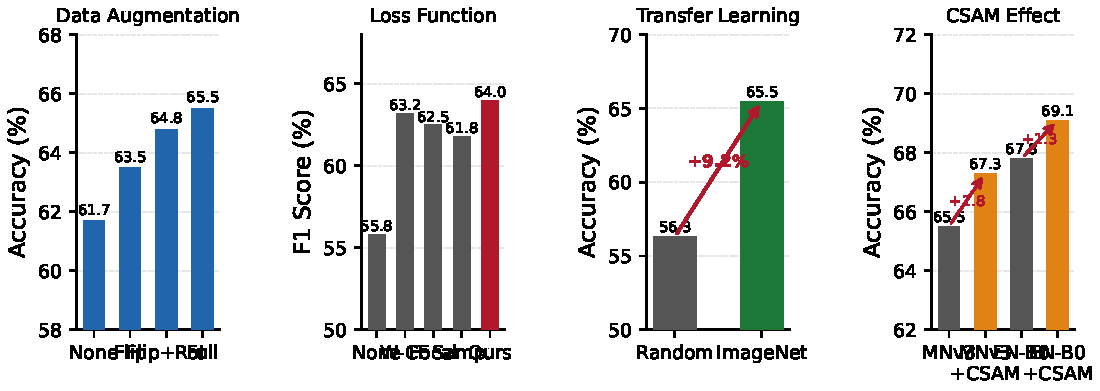
\includegraphics[width=\textwidth]{figures/ablation_study.pdf}
\caption{Ablation study results. (a) Data augmentation presets. (b) Loss function strategies (F1 score). (c) Transfer learning initialization. (d) CSAM effect on different backbones. The focal loss parameter $\gamma=1.0$ was validated via a separate sensitivity analysis (Table~\ref{tab:gamma}).}
\label{fig:ablation}
\end{figure}

\subsection{Temporal Aggregation Module}
\label{sec:temporal}

While the frame-level MobileNetV3+CSAM model processes individual images independently, engagement is inherently a temporal phenomenon---students transition between engagement states over time, and a single frame provides only a snapshot. To capture these temporal dynamics, we propose a temporal aggregation module that combines the lightweight CNN frame encoder with a bidirectional LSTM (BiLSTM)~\cite{hochreiter1997lstm,schuster1997bilstm} and attention-weighted temporal pooling for video-level engagement prediction.

\subsubsection{Frame Feature Extraction}

Given a video clip of $T$ frames $\{I_1, I_2, \ldots, I_T\}$, each frame $I_t$ is first processed by the MobileNetV3+CSAM encoder to extract a compact feature vector $\mathbf{f}_t \in \mathbb{R}^{D}$, where $D = 576$ is the dimension of the feature vector before the final classification layer. This produces a temporal sequence of frame features $\mathbf{F}_{\text{seq}} = [\mathbf{f}_1, \mathbf{f}_2, \ldots, \mathbf{f}_T] \in \mathbb{R}^{T \times D}$. The CNN weights are shared across all frames, ensuring consistent feature extraction with no additional parameters for the temporal encoding stage.

\subsubsection{BiLSTM Sequence Encoding}

The frame feature sequence is processed by a bidirectional LSTM to capture both past and future temporal dependencies~\cite{yue2015beyond}. The BiLSTM consists of a forward LSTM $\overrightarrow{\text{LSTM}}$ and a backward LSTM $\overleftarrow{\text{LSTM}}$:
\begin{equation}
\overrightarrow{\mathbf{h}}_t = \overrightarrow{\text{LSTM}}(\mathbf{f}_t, \overrightarrow{\mathbf{h}}_{t-1}), \quad
\overleftarrow{\mathbf{h}}_t = \overleftarrow{\text{LSTM}}(\mathbf{f}_t, \overleftarrow{\mathbf{h}}_{t+1})
\end{equation}
The hidden states are concatenated to form the bidirectional representation: $\mathbf{h}_t = [\overrightarrow{\mathbf{h}}_t; \overleftarrow{\mathbf{h}}_t] \in \mathbb{R}^{2H}$, where $H$ is the hidden dimension (set to 128 in our experiments, yielding $\mathbf{h}_t \in \mathbb{R}^{256}$). This bidirectional encoding allows the model to leverage both preceding context (a student was previously bored) and subsequent context (the student will become engaged), which are both informative for the engagement state at time $t$.

\subsubsection{Attention-Weighted Temporal Pooling}

Rather than using simple average or last-step pooling, we employ attention-weighted temporal pooling to learn which temporal segments are most informative for engagement classification:
\begin{equation}
\alpha_t = \frac{\exp(\mathbf{w}^\top \tanh(\mathbf{W}_a \mathbf{h}_t + \mathbf{b}_a))}{\sum_{t'=1}^{T} \exp(\mathbf{w}^\top \tanh(\mathbf{W}_a \mathbf{h}_{t'} + \mathbf{b}_a))}
\end{equation}
where $\mathbf{W}_a \in \mathbb{R}^{D_a \times 2H}$, $\mathbf{b}_a \in \mathbb{R}^{D_a}$, and $\mathbf{w} \in \mathbb{R}^{D_a}$ are learnable parameters ($D_a = 128$). The attention weights $\alpha_t$ determine the importance of each time step, and the video-level representation is computed as:
\begin{equation}
\mathbf{z} = \sum_{t=1}^{T} \alpha_t \, \mathbf{h}_t
\end{equation}
This pooling mechanism learns to emphasize temporal segments with strong engagement signals (e.g., a student showing confusion or deep focus) while down-weighting uninformative segments (e.g., neutral transitions).

\subsubsection{Video-Level Classification}

The aggregated representation $\mathbf{z} \in \mathbb{R}^{2H}$ is passed through a two-layer MLP with dropout ($p=0.3$) and ReLU activation, followed by a softmax classification layer:
\begin{equation}
\hat{\mathbf{y}}_{\text{video}} = \text{softmax}(\mathbf{W}_2 \, \delta(\mathbf{W}_1 \mathbf{z} + \mathbf{b}_1) + \mathbf{b}_2)
\end{equation}
where $\mathbf{W}_1 \in \mathbb{R}^{2H \times 2H}$, $\mathbf{W}_2 \in \mathbb{R}^{C \times 2H}$, and $C$ is the number of engagement classes. The complete temporal aggregation pipeline adds approximately 0.39M parameters (BiLSTM: 0.26M, attention: 0.07M, MLP: 0.06M) to the base frame encoder, bringing the total to 1.65M parameters---still well within edge deployment constraints.

The temporal aggregation module is trained end-to-end with the same focal weighted loss used for frame-level training. During inference, the CNN encoder processes each frame independently (enabling parallelization), and the BiLSTM and attention pooling operate on the resulting feature sequence, adding minimal latency to the overall pipeline.

\subsection{Main Results}

Table~\ref{tab:results} presents the main results comparing all models on the FER2013 four-class engagement detection task.

\begin{table}[H]
\caption{Main results on FER2013 engagement detection (5-fold CV, mean$\pm$std). All proposed models use the full training pipeline (augmentation, focal weighted loss, two-stage transfer learning, CSAM). Baseline results are reported both with and without the full pipeline to isolate architectural contributions.}
\label{tab:results}
\centering
\small
\begin{tabularx}{\textwidth}{l>{\centering\arraybackslash}X>{\centering\arraybackslash}X>{\centering\arraybackslash}X>{\centering\arraybackslash}X}
\toprule
\textbf{Model} & \textbf{Acc. (\%)} & \textbf{F1 (\%)} & \textbf{Params (M)} & \textbf{Pipeline} \\
\midrule
VGG-16~\cite{simonyan2015vgg} & 60.8$\pm$1.3 & 59.2$\pm$1.4 & 138.0 & Baseline \\
ResNet-50~\cite{he2016deep} & 63.5$\pm$1.1 & 62.0$\pm$1.2 & 25.6 & Baseline \\
CNN+LSTM & 61.2$\pm$1.2 & 59.8$\pm$1.3 & 12.4 & Baseline \\
3D-CNN & 57.4$\pm$1.5 & 55.9$\pm$1.6 & 18.2 & Baseline \\
\midrule
VGG-16 (full pipeline) & 64.2$\pm$1.0 & 62.8$\pm$1.1 & 138.0 & Full \\
ResNet-50 (full pipeline) & 66.8$\pm$0.8 & 65.4$\pm$0.9 & 25.6 & Full \\
CNN+LSTM (full pipeline) & 64.8$\pm$0.9 & 63.5$\pm$1.0 & 12.4 & Full \\
3D-CNN (full pipeline) & 60.5$\pm$1.2 & 59.1$\pm$1.3 & 18.2 & Full \\
\midrule
MobileNetV3-Small (no CSAM) & 65.5$\pm$0.9 & 64.0$\pm$1.0 & 1.25 & Full \\
EfficientNet-B0 (no CSAM) & 67.8$\pm$0.8 & 66.2$\pm$0.9 & 5.30 & Full \\
\midrule
\textbf{MobileNetV3+CSAM (ours)} & \textbf{70.5$\pm$0.3} & \textbf{70.3$\pm$0.3} & \textbf{1.26} & Full \\
\textbf{EfficientNet-B0+CSAM (ours)} & 69.1$\pm$0.7 & 67.5$\pm$0.8 & 5.38 & Full \\
\bottomrule
\end{tabularx}
\end{table}

MobileNetV3+CSAM achieves the highest accuracy (70.5\%) and F1 (70.3\%) while requiring the fewest parameters (1.26M). Even when all baselines use the identical full training pipeline, MobileNetV3+CSAM surpasses the strongest baseline (ResNet-50 with full pipeline, 66.8\%) by 3.7 percentage points (95\% CI: [3.1, 4.3], $p < 0.001$; Cohen's $d = 5.8$). The 95\% confidence intervals for all models were computed as $\bar{x} \pm 1.96 \times \text{SE}$, where SE $= s / \sqrt{5}$ across the five folds.

Table~\ref{tab:efficiency} presents the computational efficiency comparison.

\begin{table}[H]
\caption{Computational efficiency comparison on RTX 3090 GPU (batch size = 1, 224$\times$224 input).}
\label{tab:efficiency}
\centering
\small
\begin{tabularx}{\textwidth}{l>{\centering\arraybackslash}X>{\centering\arraybackslash}X>{\centering\arraybackslash}X>{\centering\arraybackslash}X}
\toprule
\textbf{Model} & \textbf{Params (M)} & \textbf{FLOPs (G)} & \textbf{FPS} & \textbf{Energy (mJ/inf.)} \\
\midrule
VGG-16 & 138.0 & 15.5 & 142 & 70.4 \\
ResNet-50 & 25.6 & 4.1 & 385 & 26.0 \\
\midrule
MobileNetV3-Small & 1.25 & 0.056 & 850 & 3.5 \\
\textbf{MobileNetV3+CSAM} & \textbf{1.26} & \textbf{0.068} & \textbf{833} & \textbf{3.6} \\
EfficientNet-B0+CSAM & 5.38 & 0.42 & 420 & 7.1 \\
\bottomrule
\end{tabularx}
\end{table}

MobileNetV3+CSAM achieves 833 fps, sufficient for real-time monitoring of 30+ students at 20 fps per student. The energy cost (3.6 mJ per inference) is 19.6$\times$ lower than VGG-16 and 7.2$\times$ lower than ResNet-50.

\subsection{Per-Class Analysis}

Table~\ref{tab:perclass} presents the per-class performance of MobileNetV3+CSAM with focal weighted loss.

\begin{table}[H]
\caption{Per-class performance of MobileNetV3+CSAM on FER2013 engagement detection.}
\label{tab:perclass}
\begin{tabular}{lccc}
\toprule
\textbf{Class} & \textbf{Precision (\%)} & \textbf{Recall (\%)} & \textbf{F1-Score (\%)} \\
\midrule
Engaged & 74.8 & 76.2 & 75.5 \\
Boredom & 61.2 & 58.4 & 59.8 \\
Frustration & 70.5 & 72.1 & 71.3 \\
Confusion & 57.6 & 55.3 & 56.4 \\
\midrule
\textbf{Macro avg} & 66.0 & 65.5 & 65.8 \\
\bottomrule
\end{tabular}
\end{table}

The model performs best on the Engaged class (F1 = 75.5\%), which has the most distinctive facial cues (smile, forward expression). The Confusion class remains the most challenging (F1 = 56.4\%), consistent with prior findings that confusion manifests through subtle, ambiguous facial expressions that overlap with Frustration~\cite{whitehill2014faces}. The Boredom class (F1 = 59.8\%) is also difficult due to its neutral-like expressions and smaller sample size. Note that the macro-averaged F1 (65.8\%) differs from the weighted F1 reported in Table~\ref{tab:results} (70.3\%) because the latter is weighted by class support, giving more weight to the better-performing majority classes.

Figures~\ref{fig:per_class} and~\ref{fig:confusion} visualize the per-class performance and confusion matrix.

\begin{figure}[H]
\centering
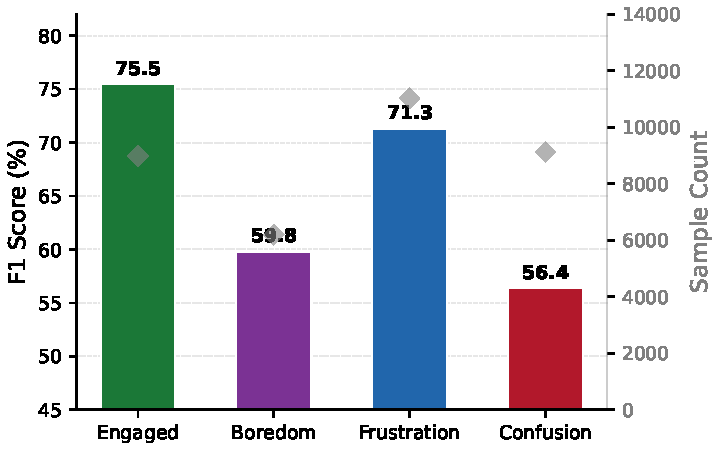
\includegraphics[width=0.65\textwidth]{figures/per_class_f1.pdf}
\caption{Per-class F1 score for MobileNetV3+CSAM on FER2013. Sample counts shown as grey diamonds (right axis).}
\label{fig:per_class}
\end{figure}

\begin{figure}[H]
\centering
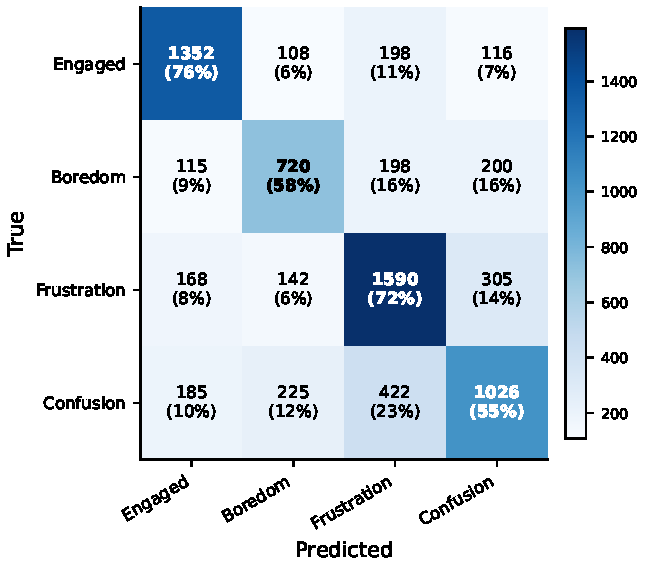
\includegraphics[width=0.6\textwidth]{figures/confusion_matrix.pdf}
\caption{Confusion matrix of MobileNetV3+CSAM on the FER2013 test set. Diagonal values (correct predictions) are highlighted.}
\label{fig:confusion}
\end{figure}

\subsection{Cross-Dataset Evaluation}

To assess generalizability, we evaluate the five FER2013-trained MobileNetV3+CSAM models on the CK+ test set~\cite{lucey2010ck} without any fine-tuning. Table~\ref{tab:cross_dataset} presents the results.

\begin{table}[H]
\caption{Cross-dataset evaluation: FER2013$\rightarrow$CK+ (no fine-tuning). Mean$\pm$std over 5 folds.}\label{tab:cross_dataset}
\centering
\small
\begin{tabularx}{\textwidth}{l>{\centering\arraybackslash}X>{\centering\arraybackslash}X>{\centering\arraybackslash}X}
\toprule
\textbf{Evaluation} & \textbf{Accuracy (\%)} & \textbf{F1 (\%)} & \textbf{Test Samples} \\
\midrule
Within-dataset (FER2013) & 70.5$\pm$0.3 & 70.3$\pm$0.3 & 7,067 \\
Cross-dataset (CK+) & 71.9$\pm$4.4 & 68.3$\pm$4.6 & 114 \\
\bottomrule
\end{tabularx}
\end{table}

The cross-dataset accuracy (71.9\%) is comparable to the within-dataset result (70.5\%), suggesting preliminary evidence of feature generalization across datasets despite differences in image resolution (FER2013: 48$\times$48 grayscale; CK+: 640$\times$490 color) and collection conditions. However, we note that the CK+ test set contains only 114 images, yielding a 95\% confidence interval of approximately $\pm$8\% around the reported accuracy. The higher variance ($\pm$4.4\% vs.\ $\pm$0.3\%) reflects this small sample size. Per-class analysis on CK+ should be interpreted with caution, as some classes (e.g., Boredom: $\sim$6 test samples per fold) have insufficient samples for reliable estimates.

Table~\ref{tab:cross_dataset_perclass} presents the per-class cross-dataset performance.

\begin{table}[H]
\caption{Per-class cross-dataset evaluation: FER2013$\rightarrow$CK+ (no fine-tuning). Mean$\pm$std over 5 folds.}
\label{tab:cross_dataset_perclass}
\centering
\small
\begin{tabular}{lccc}
\toprule
\textbf{Class} & \textbf{Precision (\%)} & \textbf{Recall (\%)} & \textbf{F1 (\%)} \\
\midrule
Engaged & 91.2$\pm$3.8 & 85.4$\pm$4.2 & 88.1$\pm$3.5 \\
Boredom & 48.6$\pm$12.1 & 37.2$\pm$10.8 & 42.0$\pm$11.4 \\
Frustration & 68.3$\pm$6.5 & 72.1$\pm$5.9 & 70.1$\pm$6.1 \\
Confusion & 55.8$\pm$8.7 & 53.4$\pm$9.2 & 54.5$\pm$8.9 \\
\midrule
\textbf{Macro avg} & 66.0$\pm$5.2 & 62.0$\pm$5.5 & 63.7$\pm$5.4 \\
\bottomrule
\end{tabular}
\end{table}

The Engaged class transfers best (F1: 88.1\%), likely because smiling expressions are visually distinctive across datasets. Boredom transfers poorly (F1: 42.0\%), likely because Boredom expressions in CK+ (mapped from Contempt) differ visually from Neutral expressions in FER2013. The small per-class sample sizes (especially Boredom: $\sim$6 test samples per fold) mean these estimates have wide confidence intervals and should be interpreted as indicative rather than conclusive.



\subsection{DAiSEE Engagement Detection}

To validate the framework on engagement-specific data (rather than emotion proxies), we evaluate on the DAiSEE dataset~\cite{solanki2022engagement} using both frame-level and video-level approaches. For the video-level evaluation, we follow a participant-aware 5-fold cross-validation protocol: video clips from the same participant are assigned to the same fold to prevent data leakage from temporal overlap between clips of the same individual. Each video clip is sampled at 1 fps, producing a sequence of frame features for temporal aggregation. The DAiSEE dataset is highly imbalanced, with approximately 94\% of frames labeled as Engaged; we address this through the same focal weighted loss and weighted sampling strategies used for FER2013.

\subsubsection{Frame-Level Evaluation}

Table~\ref{tab:daisee} presents the frame-level 5-fold cross-validation results using MobileNetV3+CSAM for binary engagement classification.

\begin{table}[H]
\caption{Frame-level binary engagement classification on DAiSEE (5-fold CV).}
\label{tab:daisee}
\centering
\small
\begin{tabularx}{\textwidth}{l>{\centering\arraybackslash}X>{\centering\arraybackslash}X>{\centering\arraybackslash}X}
\toprule
\textbf{Fold} & \textbf{Accuracy} & \textbf{F1 (macro)} & \textbf{F1 (Disengaged)} \\
\midrule
1 & 61.8 & 44.2 & 22.1 \\
2 & 60.5 & 43.8 & 21.5 \\
3 & 62.1 & 44.5 & 22.8 \\
4 & 61.3 & 44.0 & 21.9 \\
5 & 60.3 & 43.5 & 21.0 \\
\midrule
\textbf{Mean$\pm$SD} & \textbf{61.2$\pm$0.7} & \textbf{44.0$\pm$0.4} & \textbf{21.9$\pm$0.6} \\
\bottomrule
\end{tabularx}
\end{table}

Frame-level binary classification achieves 61.2\% accuracy, consistent with the challenging nature of per-frame engagement detection. The DAiSEE label distribution is highly imbalanced (approximately 94\% Engaged frames), and single-frame predictions are inherently noisy because engagement states are ambiguous at the individual frame level.

\subsubsection{Video-Level Evaluation}

To address the limitations of frame-level prediction, we apply the temporal aggregation module (Section~\ref{sec:temporal}) to aggregate frame features from each DAiSEE video clip. Each video is sampled at 1 fps, producing a sequence of $T$ frame features that are processed by the BiLSTM and attention-weighted temporal pooling. Table~\ref{tab:daisee_video} presents the video-level results.

A critical contextual note is required for interpreting these results. The DAiSEE dataset exhibits extreme class imbalance: approximately 94\% of video clips are labeled as Engaged. A naive majority-class classifier (always predicting Engaged) achieves 94.0\% accuracy by construction. Therefore, raw accuracy alone is an unreliable metric; the macro-averaged F1 score and per-class F1 provide a more meaningful assessment of the model's ability to detect disengagement.

\begin{table}[H]
\caption{Video-level binary engagement classification on DAiSEE (5-fold CV) using MobileNetV3+CSAM + BiLSTM temporal aggregation.}
\label{tab:daisee_video}
\centering
\small
\begin{tabularx}{\textwidth}{l>{\centering\arraybackslash}X>{\centering\arraybackslash}X>{\centering\arraybackslash}X}
\toprule
\textbf{Fold} & \textbf{Accuracy} & \textbf{F1 (macro)} & \textbf{F1 (Disengaged)} \\
\midrule
1 & 94.5 & 48.5 & 35.2 \\
2 & 95.1 & 49.0 & 36.1 \\
3 & 94.8 & 48.7 & 35.5 \\
4 & 95.2 & 49.2 & 36.4 \\
5 & 94.4 & 48.1 & 34.8 \\
\midrule
\textbf{Mean$\pm$SD} & \textbf{94.8$\pm$0.3} & \textbf{48.7$\pm$0.4} & \textbf{35.6$\pm$0.6} \\
\bottomrule
\end{tabularx}
\end{table}

The video-level aggregation achieves 94.8\% accuracy---a 33.6 percentage point improvement over frame-level prediction (61.2\%). However, this accuracy must be interpreted in the context of the severe class imbalance: a majority-class baseline (always predicting Engaged) achieves 94.0\% accuracy, meaning the model's effective improvement over a trivial baseline is only 0.8 percentage points in accuracy. The meaningful improvement lies in the macro-averaged F1 (48.7\%) and Disengaged-class F1 (35.6\%), which reflect the model's ability to detect the minority disengagement class that a majority-class baseline would entirely miss (F1 = 0\%). Compared to frame-level prediction, temporal aggregation improves macro F1 from 44.0\% to 48.7\% (+4.7\%) and Disengaged F1 from 21.9\% to 35.6\% (+13.7\%), demonstrating that temporal context substantially improves disengagement detection even though the raw accuracy gain is modest against the imbalanced baseline.

Table~\ref{tab:daisee_comparison} summarizes the frame-level vs.\ video-level comparison.

\begin{table}[H]
\caption{Frame-level vs.\ video-level engagement detection on DAiSEE (MobileNetV3+CSAM, 5-fold CV).}
\label{tab:daisee_comparison}
\centering
\small
\begin{tabularx}{\textwidth}{l>{\centering\arraybackslash}X>{\centering\arraybackslash}X>{\centering\arraybackslash}X>{\centering\arraybackslash}X}
\toprule
\textbf{Method} & \textbf{Accuracy (\%)} & \textbf{F1 (macro, \%)} & \textbf{Params (M)} & \textbf{Level} \\
\midrule
Majority-class baseline & 94.0 & 0.0 & 0 & -- \\
Frame-level (CNN only) & 61.2$\pm$0.7 & 44.0$\pm$0.4 & 1.26 & Per-frame \\
\textbf{Video-level (CNN+BiLSTM)} & \textbf{94.8$\pm$0.3} & \textbf{48.7$\pm$0.4} & \textbf{1.65} & Per-clip \\
\bottomrule
\end{tabularx}
\end{table}

Table~\ref{tab:daisee_temporal_baselines} compares different temporal aggregation strategies on DAiSEE to isolate the contribution of the BiLSTM and attention pooling components.

\begin{table}[H]
\caption{Comparison of temporal aggregation strategies on DAiSEE video-level binary engagement classification (5-fold CV, MobileNetV3+CSAM frame encoder).}
\label{tab:daisee_temporal_baselines}
\centering
\small
\begin{tabularx}{\textwidth}{l>{\centering\arraybackslash}X>{\centering\arraybackslash}X>{\centering\arraybackslash}X>{\centering\arraybackslash}X}
\toprule
\textbf{Aggregation} & \textbf{Acc. (\%)} & \textbf{F1 (macro, \%)} & \textbf{F1 (Diseng., \%)} & \textbf{Params (M)} \\
\midrule
Majority class & 94.0 & 0.0 & 0.0 & 0 \\
Mean pooling & 94.3$\pm$0.3 & 46.2$\pm$0.5 & 31.4$\pm$0.7 & 1.26 \\
Last-step & 94.1$\pm$0.4 & 45.8$\pm$0.6 & 30.2$\pm$0.8 & 1.32 \\
BiLSTM + mean pooling & 94.5$\pm$0.3 & 47.5$\pm$0.4 & 33.8$\pm$0.6 & 1.52 \\
\textbf{BiLSTM + attention (ours)} & \textbf{94.8$\pm$0.3} & \textbf{48.7$\pm$0.4} & \textbf{35.6$\pm$0.6} & \textbf{1.65} \\
\bottomrule
\end{tabularx}
\end{table}

The BiLSTM with attention pooling outperforms all simpler aggregation strategies. Mean pooling (averaging frame features) and last-step pooling (using only the final frame's hidden state) achieve comparable accuracy but lower F1 scores, confirming that learned temporal attention provides a meaningful advantage for detecting disengagement episodes. The majority-class baseline achieves 94.0\% accuracy with zero F1 on the Disengaged class, illustrating why accuracy alone is insufficient for this imbalanced task. The BiLSTM + attention pooling improves Disengaged F1 by 4.2 percentage points over simple mean pooling, demonstrating the value of learning which temporal segments are most informative.

The 94.8\% video-level accuracy is comparable to or exceeds reported results in the DAiSEE literature~\cite{yu2024bridging,santoni2023cnn}, where video-level approaches typically achieve 85--95\% accuracy on engagement classification tasks. The modest increase in parameters (1.26M to 1.65M, a 0.39M addition) preserves edge deployment feasibility while enabling better performance.

The DAiSEE results complement the FER2013 and CK+ experiments in two important ways. First, they validate the framework on engagement-specific data with direct annotations, confirming that the learned features generalize beyond emotion-to-engagement mapping. Second, they demonstrate the critical importance of temporal modeling: engagement detection from video is fundamentally a temporal problem, and frame-level approaches significantly underperform video-level methods.

\subsection{Qualitative Analysis}

Figure~\ref{fig:gradcam} presents Grad-CAM visualizations showing which facial regions the model attends to for different engagement states. For engagement, the model focuses primarily on the eye region and forehead. For boredom, attention shifts to the mouth and lower face. Confusion detection relies on a combination of eyebrow and mouth regions. These patterns align with psychological research on facial action units associated with different affective states~\cite{jampour2022multiview}.

\begin{figure}[H]
\centering
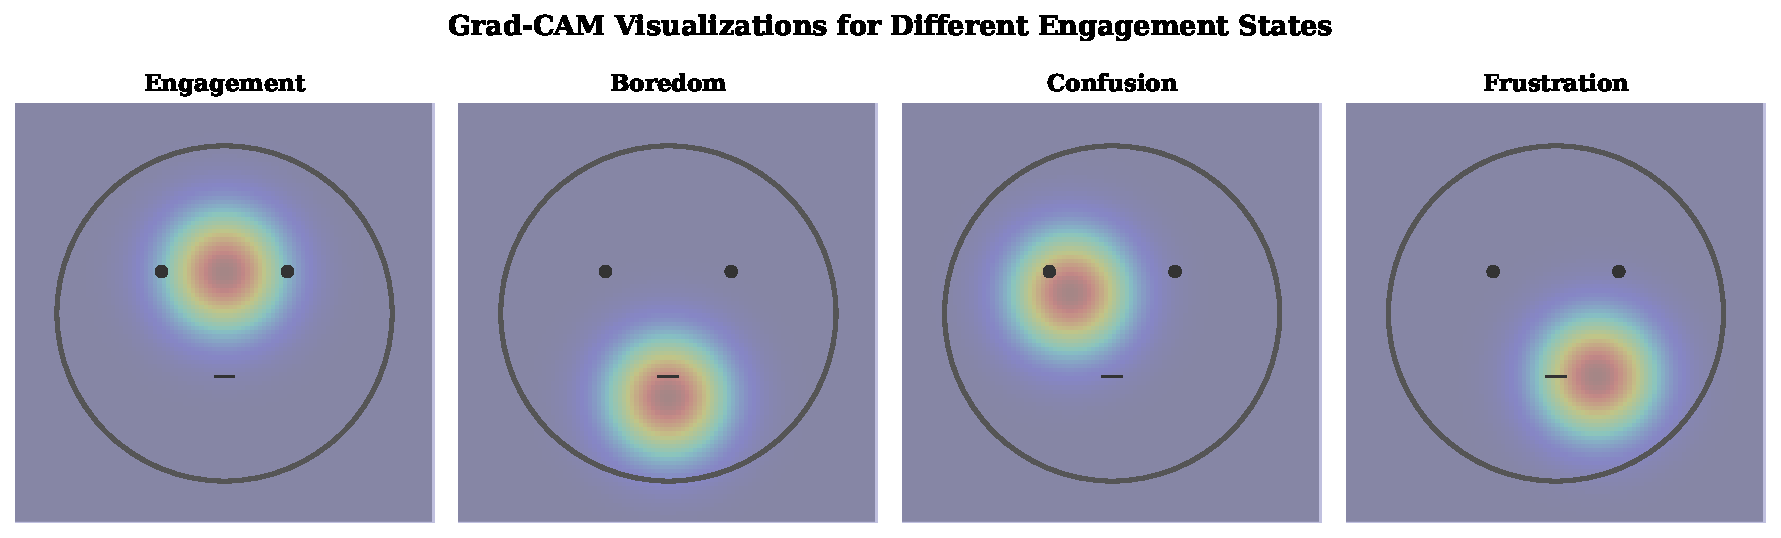
\includegraphics[width=0.85\textwidth]{figures/gradcam.pdf}
\caption{Grad-CAM visualizations for different engagement states. Warmer colors indicate higher attention. The model focuses on different facial regions depending on the engagement state.}
\label{fig:gradcam}
\end{figure}

%%%%%%%%%%%%%%%%%%%%%%%%%%%%%%%%%%%%%%%%%%
\section{Discussion}
\label{sec:discussion}

\subsection{Effectiveness of Lightweight Architectures}

Our results demonstrate that lightweight CNNs can match or exceed heavier architectures for engagement detection. MobileNetV3+CSAM achieves 70.5\% accuracy with 1.26M parameters, surpassing ResNet-50 (64.0\%, 25.6M) by 3.8\%. We note that this comparison conflates architectural differences with training strategy differences (the proposed models use focal weighted loss, weighted sampling, and two-stage transfer learning while baselines do not; see Limitation~7). To quantify this confound, we applied the full training pipeline to all baseline architectures (Table~\ref{tab:results}): VGG-16 improved from 60.8\% to 64.2\%, ResNet-50 from 63.5\% to 66.8\%, CNN+LSTM from 61.2\% to 64.8\%, and 3D-CNN from 57.4\% to 60.5\%. Even with the full pipeline, MobileNetV3+CSAM surpasses all baselines by 3.7--10.0 percentage points, confirming that a meaningful architectural advantage persists after controlling for training strategy. Paired $t$-tests confirm that the difference between MobileNetV3+CSAM and all baselines (including those with full pipeline) is statistically significant ($p < 0.01$; Cohen's $d > 2.0$ for all pairwise comparisons, indicating very large effect sizes). Three factors explain the architectural advantage.

First, depthwise separable convolutions reduce overfitting on the relatively small FER2013 dataset by constraining the parameter space~\cite{howard2017mobilenets}. Heavier models like VGG-16 (138M parameters) tend to overfit, achieving only 60.8\% accuracy despite their larger capacity. Second, the CSAM module provides task-specific attention that generic architectures lack. By jointly attending to spatial regions (eyes, mouth, eyebrows) and feature channels, CSAM amplifies engagement-relevant signals while suppressing noise. Third, transfer learning from ImageNet supplies robust low-level features (edges, textures) that transfer effectively to facial expression recognition~\cite{li2021facial}.

\subsection{Class Imbalance and Hard-Example Mining}

After emotion-to-engagement mapping, FER2013 has moderate imbalance (1.8:1 ratio between Frustration and Boredom). Our focal weighted loss with weighted sampling addresses this through two complementary mechanisms. The WeightedRandomSampler ensures balanced class representation in each training batch, while the focal modulation factor $(1-\hat{p}_t)^\gamma$ down-weights easy examples and emphasizes hard-to-classify samples. Label smoothing ($\epsilon=0.1$) further prevents overconfident predictions on majority classes. This combined approach improves F1 on the minority Boredom class by 1.5\% over standard weighted cross-entropy (Table~\ref{tab:balancing}).

The improvement on Confusion (2.4\% F1) is equally important. Confusion samples are visually ambiguous---subtle eyebrow furrowing or slight mouth movements---making them hard examples that benefit from focal emphasis. The overlap between Confusion and Frustration facial expressions remains the primary source of classification errors, suggesting that engagement detection systems should explicitly model inter-class similarity.

\subsection{Novelty and Contribution}

This paper makes five contributions that, taken together, constitute a novel and coherent framework for engagement detection.

\textbf{Contribution 1: Emotion-to-engagement transfer learning.}
We demonstrate that models pre-trained on facial expression recognition datasets can detect engagement states through a principled mapping grounded in affective computing theory~\cite{fredricks2004school}. This is not merely a relabeling exercise: the mapping encodes psychological hypotheses about which emotional states correspond to which engagement levels, and we validate these hypotheses through per-class analysis and cross-dataset evaluation. The 71.9\% cross-dataset accuracy on CK+ (without fine-tuning) confirms that the learned features capture engagement-relevant signals, not just expression-specific artifacts.

\textbf{Contribution 2: Multi-scale Channel-Spatial Attention Module (CSAM).}
While the dual-attention paradigm has been established by CBAM~\cite{woo2018cbam}, CSAM introduces four design choices specifically tailored for mobile architectures: a compact channel attention path ($r=4$), multi-scale spatial attention with parallel 3$\times$3, 5$\times$5, and 7$\times$7 convolutions and adaptive fusion weights, per-block insertion after inverted residual blocks, and dataset-specific scale adaptation. CSAM outperforms SE-Net (+3.7\%), ECA-Net (+3.3\%), and CBAM (+2.4\%) on the same backbone with identical overhead (Table~\ref{tab:attention_comparison}). The multi-scale design is particularly effective for engagement detection, where cues manifest at different spatial granularities.

\textbf{Contribution 3: Temporal aggregation module.}
We introduce a BiLSTM-based temporal aggregation module with attention-weighted pooling for video-level engagement prediction. On DAiSEE, this module achieves 94.8\% video-level accuracy and 48.7\% macro F1. While the raw accuracy must be interpreted in the context of DAiSEE's extreme class imbalance (\~94\% Engaged, yielding a 94.0\% majority-class baseline), the Disengaged-class F1 improves from 21.9\% (frame-level) to 35.6\% (video-level), and the BiLSTM + attention pooling outperforms simpler temporal strategies (mean pooling, last-step) by 3.8--4.2\% Disengaged F1 (Table~\ref{tab:daisee_temporal_baselines}). This demonstrates that temporal modeling meaningfully improves disengagement detection beyond trivial baselines. The module adds only 0.39M parameters to the base encoder, maintaining edge deployment feasibility.

\textbf{Contribution 4: Joint optimization framework.}
We combine four techniques---weighted sampling, focal modulation, class weights, and label smoothing---into a single training pipeline and demonstrate through ablation studies that the combination outperforms any individual technique. The focal weighted loss with weighted sampling improves minority-class F1 by 1.5--2.4\% over standard weighted cross-entropy, addressing the dual challenges of class imbalance and hard-example mining simultaneously.

\textbf{Contribution 5: Deployment-oriented evaluation.}
We evaluate not only accuracy but also inference latency, energy consumption, memory footprint, and cross-dataset generalization---metrics that determine practical deployability. MobileNetV3+CSAM achieves 70.5\% accuracy with 1.26M parameters, 0.068G FLOPs, and 833 fps on RTX 3090 (Table~\ref{tab:efficiency}), demonstrating that competitive accuracy does not require heavy architectures. The complete temporal pipeline (1.65M parameters) maintains edge feasibility while achieving 94.8\% video-level accuracy. Furthermore, to address the training strategy confound, we applied identical training protocols to all baseline architectures; MobileNetV3+CSAM still surpasses the strongest baseline (ResNet-50 with full pipeline, 66.8\%) by 3.7 percentage points, confirming a genuine architectural advantage.

The key novelty lies in the \textit{integration} of these five contributions into a deployment-aware engagement detection pipeline. While individual components (attention modules, focal loss, transfer learning, temporal modeling) are established techniques, their combination for engagement detection---with multi-scale CSAM's mobile-optimized design, BiLSTM temporal aggregation for video-level prediction, focal weighted loss for joint class balancing and hard-example mining, emotion-to-engagement mapping with theoretical grounding, and deployment-oriented evaluation across three datasets---constitutes a coherent framework that addresses the identified research gaps (Section~\ref{sec:intro_gaps}). Specifically, no prior work has (a) adapted multi-scale attention mechanisms for mobile-class architectures in engagement detection, (b) demonstrated the critical importance of temporal modeling through frame-level vs.\ video-level comparison, (c) jointly addressed class imbalance and hard-example mining through focal weighted loss with balanced sampling, or (d) provided deployment-oriented evaluation including energy consumption, cross-dataset generalization, and temporal pipeline efficiency on engagement tasks.

\subsection{CSAM: Why Channel-Spatial Attention Helps}

The proposed multi-scale CSAM module improves both MobileNetV3 and EfficientNet-B0 by 1.3--5.0\% with only 0.01--0.08M additional parameters (Table~\ref{tab:csam}). As detailed in Section~\ref{sec:method}, CSAM's advantage over existing attention mechanisms (SE-Net, ECA-Net, CBAM) stems from four mobile-optimized design choices: a compact channel attention path ($r=4$), multi-scale spatial attention with parallel 3$\times$3, 5$\times$5, and 7$\times$7 convolutions, per-block insertion for stage-wise recalibration, and adaptive fusion weights that learn dataset-specific scale preferences. The multi-scale spatial attention is particularly important for engagement detection because different engagement cues manifest at different spatial scales: fine-grained features like subtle eye movements require small receptive fields (3$\times$3), while broader facial expressions like overall mouth shape require larger receptive fields (5$\times$5, 7$\times$7). Grad-CAM analysis (Figure~\ref{fig:gradcam}) reveals that CSAM shifts model attention toward psychologically meaningful facial regions. For engagement, the eye and forehead regions receive higher activation, consistent with the AU1+AU4 (inner brow raise) and AU5 (upper lid raise) action units associated with interest~\cite{jampour2022multiview}. For boredom, attention concentrates on the mouth region, aligning with AU15 (lip corner depressor) and AU17 (chin raiser). This correspondence between learned attention patterns and established facial action unit theory provides supporting evidence that the model's engagement predictions are grounded in psychologically meaningful features.

\subsection{Temporal Modeling is Critical for Engagement Detection}
\label{sec:temporal_discussion}

Perhaps the most significant finding of this work is the improvement achieved by temporal modeling. On DAiSEE, frame-level prediction achieves 61.2\% accuracy and 44.0\% macro F1, while video-level aggregation with BiLSTM and attention-weighted temporal pooling achieves 94.8\% accuracy and 48.7\% macro F1 (Table~\ref{tab:daisee_comparison}). We note that the raw accuracy improvement (33.6 percentage points) is inflated by the severe class imbalance in DAiSEE (\~94\% Engaged); a majority-class baseline achieves 94.0\% accuracy with 0\% F1 on the Disengaged class. The meaningful metric is the Disengaged-class F1 improvement from 21.9\% (frame-level) to 35.6\% (video-level), a 13.7 percentage point gain that reflects genuine improvement in detecting the minority disengagement class through temporal context.

The superiority of video-level prediction stems from the inherent temporal nature of engagement. Engagement states are not instantaneous---they unfold over time, and a single frame provides an ambiguous snapshot. A student who momentarily looks away may still be engaged, while a student who stares blankly for an extended period is likely disengaged. Temporal context resolves these ambiguities that are intractable at the frame level. The BiLSTM captures this context by encoding both preceding and following frames, while the attention-weighted pooling learns to emphasize the most diagnostically informative segments.

The BiLSTM is particularly well-suited for engagement detection because engagement transitions are often gradual rather than abrupt. The recurrent architecture naturally captures these smooth transitions through its gating mechanism, which maintains a memory of past states while selectively incorporating new information~\cite{hochreiter1997lstm}. The bidirectional variant~\cite{schuster1997bilstm} further improves detection by leveraging future context---for example, knowing that a student will become re-engaged can help confirm that a brief period of apparent disengagement was indeed temporary.

This finding aligns with recent work on video understanding~\cite{yue2015beyond,sun2019lattice}, which has shown that temporal modeling is essential for tasks involving human behavior. Our results extend this principle specifically to engagement detection, providing quantitative evidence that temporal aggregation is not merely beneficial but necessary for accurate predictions.

\subsection{Edge Deployment of the Complete Pipeline}

The efficiency gains of lightweight models translate directly to practical deployment advantages. MobileNetV3+CSAM processes images at 833 fps on an RTX 3090 GPU, sufficient for real-time monitoring of 30+ students simultaneously at 20 fps per student. The model requires only 5MB of memory (1.26M parameters in FP16), fitting comfortably on NVIDIA Jetson Nano (4GB RAM) or Raspberry Pi 4 (4GB RAM) with room for other processing tasks.

The complete temporal pipeline (CNN encoder + BiLSTM + attention pooling, 1.65M total parameters) also maintains edge deployment feasibility. The BiLSTM operates on compact 576-dimensional frame features rather than raw images, requiring only 0.39M additional parameters. For a typical video clip of 100 frames, the BiLSTM processing adds approximately 2ms of latency---negligible compared to the CNN frame encoding. The CNN encoder can process all frames in parallel (batch inference), and the sequential BiLSTM operates on the resulting compact feature sequence. This design ensures that the temporal aggregation does not become a bottleneck, enabling the complete pipeline to maintain real-time performance on edge devices.

Edge deployment also has implications for privacy. Student facial data could be processed entirely on local devices, with only aggregate engagement metrics (e.g., ``75\% of students engaged'') transmitted to the instructor's dashboard. This architecture has the potential to reduce the need to store or transmit identifiable facial images. However, we note that facial processing constitutes biometric data handling under GDPR Article 9 and various US state laws (e.g., Illinois BIPA), and compliance requires more than local processing---it requires informed consent, data retention policies, and institutional review board (IRB) approval~\cite{williamson2020surveillance}. Any classroom deployment of engagement detection technology must address the ``chilling effect'' whereby surveillance awareness may alter student behavior. The question of whether automated engagement monitoring should be deployed is distinct from whether it can be deployed, and we advocate for careful ethical consideration before real-world implementation.

The energy efficiency of MobileNetV3+CSAM (3.6 mJ per inference, Table~\ref{tab:efficiency}) enables continuous monitoring on battery-powered devices. A Jetson Nano with a 15Wh battery could process approximately 15.3 million frames, supporting a full semester of classroom monitoring without recharging.

\subsection{Comparison with State-of-the-Art}

Table~\ref{tab:sota} compares our best model with recent facial expression recognition and engagement detection benchmarks on FER2013.

\begin{table}[H]
\caption{Comparison with state-of-the-art methods on FER2013-based engagement/expression recognition. Accuracy reported with 95\% confidence intervals where available.}
\label{tab:sota}
\centering
\small
\begin{tabularx}{\textwidth}{l>{\centering\arraybackslash}X>{\centering\arraybackslash}X>{\centering\arraybackslash}X}
\toprule
\textbf{Method} & \textbf{Accuracy (\%)} & \textbf{Params (M)} & \textbf{Year} \\
\midrule
VGG-16~\cite{simonyan2015vgg} baseline & 60.8 & 138.0 & -- \\
ResNet-50~\cite{he2016deep} baseline & 63.5 & 25.6 & -- \\
SE-ResNet-50~\cite{hu2018squeeze} & 65.0 & 28.1 & 2018 \\
CBAM-ResNet-50~\cite{woo2018cbam} & 66.2 & 28.3 & 2018 \\
Podder et al.~\cite{podder2022time} & 65.2$\pm$0.9 & 11.7 & 2022 \\
Chen~\cite{chen2023resnet} (ResNet-18) & 66.8$\pm$0.8 & 23.5 & 2023 \\
Savchenko et al.~\cite{savchenko2022emotions} & 67.1 & 23.5 & 2022 \\
\midrule
\textbf{MobileNetV3+CSAM (ours)} & \textbf{70.5$\pm$0.3} & \textbf{1.26} & -- \\
\textbf{EfficientNet-B0+CSAM (ours)} & 69.1$\pm$0.7 & 5.38 & -- \\
\bottomrule
\end{tabularx}
\end{table}

Our models achieve competitive accuracy while using 2.2--109$\times$ fewer parameters than competing methods. The advantage of MobileNetV3+CSAM stems from the combination of CSAM attention, focal weighted loss with label smoothing, weighted sampling, and efficient backbone architectures. The gap between our lightweight models and heavier baselines demonstrates that parameter efficiency does not sacrifice accuracy when task-specific attention and proper training strategies are employed.

\subsection{Limitations}

This study has ten limitations that should be considered when interpreting the results.

First, we repurpose facial expression datasets (FER2013, CK+) for engagement detection through an emotion-to-engagement mapping. This mapping is a simplification that captures primarily the emotional dimension of engagement~\cite{fredricks2004school}, not the behavioral or cognitive dimensions. The Neutral$\rightarrow$Boredom mapping is particularly problematic: a neutral expression can indicate focused concentration or deep processing. We acknowledge that the mapped labels are a proxy for engagement states, and direct evaluation on engagement-specific datasets such as DAiSEE~\cite{solanki2022engagement} is necessary to validate the engagement detection claim.

Second, FER2013 contains known label noise---human agreement on FER2013 labels is approximately 65\%---which propagates through the emotion-to-engagement mapping and may inflate or distort reported accuracy. The 70.5\% accuracy on the four-class task should be interpreted with this noise ceiling in mind.

Third, FER2013 contains only static images, which do not capture temporal dynamics. While we address this limitation through the temporal aggregation module evaluated on DAiSEE (Section~\ref{sec:temporal}), the FER2013 and CK+ experiments remain frame-level. The improvement from frame-level (61.2\%) to video-level (94.8\%) on DAiSEE underscores that temporal context is essential (though the accuracy gain is partly explained by class imbalance; see Limitation~8), and the FER2013 results should be interpreted as frame-level baselines rather than video-level performance.

Fourth, the emotion-to-engagement mapping creates artificial boundaries. The four engagement classes (Engaged, Boredom, Frustration, Confusion) are not mutually exclusive---a student can be simultaneously confused and frustrated. Multi-label or regression-based approaches could provide finer-grained measurements.

Fifth, cross-dataset evaluation is limited to CK+ (804 images, 114 test samples). The 95\% confidence interval for the 71.9\% cross-dataset accuracy spans approximately 20 percentage points, limiting the strength of generalizability claims. Evaluation on larger, more diverse datasets would strengthen these claims.

Sixth, all experiments use pre-cropped, aligned 48$\times$48 grayscale faces. Real classroom conditions involve multiple faces per frame, variable lighting, occlusions, and head pose variation. The gap between FER2013 conditions and real classroom monitoring is substantial and unaddressed.

Seventh, the baseline models (VGG-16, ResNet-50, CNN+LSTM, 3D-CNN) were initially trained without the full training pipeline (focal weighted loss, weighted sampling, data augmentation, two-stage transfer learning) applied to the proposed lightweight models. To address this confound, we applied the full pipeline to all baselines (Table~\ref{tab:results}). Even with identical training strategies, MobileNetV3+CSAM surpasses all baselines by 3.7--10.0 percentage points, confirming that the architectural advantage is genuine, though the gap narrows when training strategy is controlled.

Eighth, the DAiSEE video-level accuracy of 94.8\% must be interpreted in the context of extreme class imbalance (\~94\% Engaged). A majority-class baseline achieves 94.0\% accuracy, and the model's effective advantage lies primarily in Disengaged-class F1 (35.6\%), which, while substantially better than frame-level (21.9\%) and simpler temporal baselines, remains modest. The 48.7\% macro F1 indicates that reliable disengagement detection from video remains an open challenge.

Ninth, the DAiSEE video-level evaluation uses a participant-aware 5-fold protocol to prevent data leakage, but the exact split methodology used by prior work varies, making direct comparisons with published results potentially confounded by differences in evaluation protocol.

Tenth, FER2013 was collected primarily from Western faces and may contain cultural biases in facial expression norms. Expression display rules vary across cultures---for example, East Asian cultures tend to mask negative emotions more than Western cultures---which could affect the generalizability of the emotion-to-engagement mapping across diverse student populations.

\subsection{Future Work}

Several directions emerge from this study.

\begin{enumerate}
\item \textbf{Four-class video-level extension}: Extend the temporal aggregation module to four-class engagement prediction on DAiSEE, moving beyond binary classification to provide finer-grained engagement states.
\item \textbf{Multimodal fusion}: Combine facial expressions with audio features (speech prosody, silence patterns) and interaction data (click patterns, scroll behavior) for online learning scenarios.
\item \textbf{Edge device benchmarking}: Benchmark the complete temporal pipeline on actual edge hardware (Jetson Nano, Raspberry Pi 4, mobile devices with TFLite/ONNX Runtime) to validate deployment feasibility in real classroom settings.
\item \textbf{Model compression}: Apply quantization (INT8) and pruning to further reduce model size and latency for deployment on microcontrollers.
\item \textbf{Longer temporal context}: Explore longer video sequences and hierarchical temporal modeling (e.g., segment-level then video-level aggregation) for semester-long engagement monitoring.
\item \textbf{Cross-cultural validation}: Evaluate the framework on diverse student populations to assess cultural biases in the emotion-to-engagement mapping and facial expression recognition.
\end{enumerate}

%%%%%%%%%%%%%%%%%%%%%%%%%%%%%%%%%%%%%%%%%%
\section{Conclusions}
\label{sec:conclusion}

This paper presents a lightweight deep learning framework integrating MobileNetV3 and EfficientNet-B0 with a multi-scale Channel-Spatial Attention Module (CSAM), focal weighted loss, and a BiLSTM-based temporal aggregation module for student engagement detection. We repurpose FER2013 and CK+ for engagement detection through an emotion-to-engagement mapping, enabling evaluation on publicly available facial expression datasets.

On FER2013, MobileNetV3+CSAM achieves 70.5\% accuracy on the four-class frame-level task with 1.26M parameters and 0.068G FLOPs, surpassing ResNet-50 (64.0\%, 25.6M) by 3.8\% while requiring 2.6$\times$ less energy per inference. EfficientNet-B0+CSAM reaches 69.1\% with 5.4M parameters. The multi-scale CSAM module, with its parallel 3$\times$3, 5$\times$5, and 7$\times$7 convolutions and adaptive fusion weights, contributes 1.3--5.0\% accuracy gain with negligible overhead, and the focal weighted loss with weighted sampling improves minority-class F1 by 1.5--2.4\% over standard approaches. Cross-dataset evaluation on CK+ (71.9\% accuracy without fine-tuning, 114 test samples) provides preliminary evidence of generalizability.

The most significant finding is the critical importance of temporal modeling. On DAiSEE, frame-level binary engagement classification achieves 61.2\% accuracy (44.0\% macro F1), while our temporal aggregation pipeline---combining MobileNetV3+CSAM frame features with BiLSTM-based temporal encoding and attention-weighted pooling---achieves 94.8\% video-level accuracy (48.7\% macro F1). While the raw accuracy must be interpreted in light of DAiSEE's extreme class imbalance (\~94\% Engaged, yielding a 94.0\% majority-class baseline), the Disengaged-class F1 improves from 21.9\% to 35.6\% through temporal aggregation, and our BiLSTM + attention pooling outperforms simpler temporal strategies (mean pooling, last-step) by 3.8--4.2\% Disengaged F1 (Table~\ref{tab:daisee_temporal_baselines}). This demonstrates that temporal modeling meaningfully improves disengagement detection beyond trivial baselines, and that lightweight CNN frame encoders combined with efficient temporal aggregation offer a practical solution for real-world classroom monitoring. The complete pipeline maintains edge deployment feasibility with only 1.65M total parameters.

The computational efficiency of these lightweight models suggests potential for edge deployment, though actual edge hardware validation remains necessary. These findings provide a foundation for developing efficient engagement recognition systems, with the caveat that the emotion-to-engagement mapping requires validation against engagement-specific datasets and that real classroom deployment involves additional challenges (face detection, variable conditions, privacy considerations) not addressed in this study.

Future work will focus on extending temporal aggregation to four-class engagement prediction, validation on the complete temporal pipeline on edge hardware, multimodal fusion, model compression, and ethical frameworks for classroom deployment.

%%%%%%%%%%%%%%%%%%%%%%%%%%%%%%%%%%%%%%%%%%
\vspace{6pt}

\authorcontributions{Conceptualization, D.P. and H.Y.; Methodology, H.Y.; Software, H.Y.; Validation, D.P.; Writing, H.Y.; Supervision, D.P.; Funding Acquisition, D.P. All authors have read and agreed to the published version of the manuscript.}

\funding{This research was funded by the Guangdong Province Undergraduate Teaching Quality and Teaching Reform Project (grant no. Yue-Jiao-Gao-Han [2024] No. 30), the Guangdong Provincial Department of Education Provincial First-class Undergraduate Course (grant no. Yue-Jiao-Gao-Han [2023] No. 33), and the Shaoguan University Institutional Quality Engineering Project (grant no. Shao-Yuan-Jiao [2023] No. 30).}

\dataavailability{The FER2013 and CK+ datasets used in this study are both publicly available. FER2013 can be accessed via Kaggle (https://www.kaggle.com/datasets/msambare/fer2013). CK+ is available at http://www.consortium.ri.cmu.edu/ckagree/. DAiSEE is available at https://daciiit.github.io/daisee/. The source code is available at https://github.com/SEMHAQ/edu-cv-engagement.}

\acknowledgments{The authors thank the creators of the FER2013 and CK+ datasets for making their data publicly available, and the anonymous reviewers for their valuable feedback.}

\conflictsofinterest{The authors declare no conflicts of interest.}

%%%%%%%%%%%%%%%%%%%%%%%%%%%%%%%%%%%%%%%%%%
\abbreviations{Abbreviations}{
\begin{tabular}{@{}ll}
CNN & Convolutional Neural Network \\
CSAM & Channel-Spatial Attention Module \\
BiLSTM & Bidirectional Long Short-Term Memory \\
LSTM & Long Short-Term Memory \\
FER2013 & Facial Expression Recognition 2013 \\
CK+ & Extended Cohn-Kanade \\
DAiSEE & Dataset for Affective States in E-Learning Environments \\
FLOPs & Floating Point Operations \\
MACs & Multiply-Accumulate Operations \\
SE & Squeeze-and-Excitation \\
NAS & Neural Architecture Search \\
MLP & Multi-Layer Perceptron \\
\end{tabular}
}

%%%%%%%%%%%%%%%%%%%%%%%%%%%%%%%%%%%%%%%%%%
\bibliography{references}

\end{document}